\documentclass[amsmath,secnumarabic,floatfix,amssymb,nofootinbib,nobibnotes,letterpaper,11pt,tightenlines,showkeys]{revtex4}

\usepackage{times}

\usepackage{geometry}
\usepackage{amssymb}
\usepackage{latexsym, amsmath, amscd,amsthm}
\usepackage{graphicx}
\usepackage{array}
\usepackage[percent]{overpic}
%\usepackage{pdfsync}
\usepackage{units}
\usepackage{hyperref}
\PassOptionsToPackage{caption=false}{subfig}
\usepackage[lofdepth]{subfig}

\usepackage{clrscode}

\def\figdir{figs/}
\graphicspath{\figdir}

\newtheorem{theorem}{Theorem}
\newtheorem*{maintheorem}{Main Theorem}
\newtheorem{lemma}[theorem]{Lemma}
\newtheorem{proposition}[theorem]{Proposition}
\newtheorem{corollary}[theorem]{Corollary}

\theoremstyle{definition}
\newtheorem{definition}[theorem]{Definition}
\newtheorem*{example}{Example}
\newtheorem{conjecture}[theorem]{Conjecture}
\newtheorem{remark}[theorem]{Remark}

\def\defn#1{Definition~\ref{def:#1}}
\def\thm#1{Theorem~\ref{thm:#1}}
\def\lem#1{Lemma~\ref{lem:#1}}
\def\figr#1{Figure~\ref{fig:#1}}
\def\prop#1{Proposition~\ref{prop:#1}}
\def\cor#1{Corollary~\ref{cor:#1}}
\def\sect#1{Section~\ref{sect:#1}}
\def\mainthm#1{Main Theorem~\ref{mainthm:#1}}
\def\mainthm#1{Main Theorem~\ref{mainthm:#1}}
\def\rmark#1{Remark~\ref{rmark:#1}}
%\numberwithin{equation}{section}

% make a small change

\newcommand{\abs}[1]{\lvert#1\rvert}
\newcommand{\tvnorm}[1]{\left| #1 \right|_{\operatorname{TV}}}
\newcommand{\R}{\mathbb{R}}
\newcommand{\C}{\mathbb{C}}
\newcommand{\Q}{\mathbb{H}}
\newcommand{\Z}{\mathbb{Z}}
\newcommand{\F}{\mathbb{F}}

\newcommand{\arc}[1]{\gamma_{#1}}
\newcommand{\len}[1]{\ell_{#1}}
\newcommand{\bdry}{\partial}
\newcommand{\bdy}{\bdry}
\newcommand{\isom}{\cong}
\newcommand{\setm}{\smallsetminus}
\newcommand{\eps}{\varepsilon}
\newcommand{\lk}{\textrm{lk}}
\newcommand{\intr}{\textrm{int}} %interior
\newcommand{\half}{\tfrac12}
\newcommand{\arcsec}{\textrm{arcsec}}
\newcommand{\m}{\mathcal}
\renewcommand{\d}{\partial}
\newcommand{\grad}{\nabla}
\newcommand{\PThree}{\ePol_3(n)/\SO(3)}
\newcommand{\EOne}{E_1}
\newcommand{\ETwo}{E_2}
\newcommand{\FOne}{F_1}

\newcommand{\loopinsert}{E_1}
\newcommand{\edgedouble}{E_2}
\newcommand{\cutedgedouble}{E_3}
\newcommand{\pairinsert}{E_4}
\newcommand{\plantri}{\texttt{plantri} }

\graphicspath{{../../figs/}{figs/}}

\bibliographystyle{plain}
%
\def\co{\colon\!}

\setlength{\parskip}{5pt}

\let\mgp=\marginpar \marginparwidth18mm \marginparsep1mm
\def\marginpar#1{\mgp{\raggedright\tiny #1}}
%\def\marginpar#1{}   %Uncomment this to hide all marginpars

\let\lbl=\label
\def\label#1{\lbl{#1}\ifinner\else\marginpar{\ref{#1} #1}\ignorespaces\fi}

\bibliographystyle{plain}

\begin{document}
\title[]{Knot Probabilities in Random Diagrams}
\author{Jason Cantarella, Harrison Chapman, Eric Lybrand, Hollis Neel and Malik Henry}
\altaffiliation{University of Georgia, Mathematics Department, Athens GA}
\noaffiliation
\author{Matt Mastin}
\altaffiliation{Wake Forest University, Mathematics Department, Athens GA}
\noaffiliation
\author{Eric Rawdon(?)}
\altaffiliation{Wake Forest University, Mathematics Department, Athens GA}
\noaffiliation

\maketitle

Suppose that one is given an $n$-crossing knot diagram chosen at random from the (finite) set of such diagrams. What is the probability that it is a diagram of the unknot? In this paper, we report on a computer experiment which gives precise answers to this and similar questions for $n \leq 12$ by direct enumeration and classification of knot diagrams. From the point of view of classical knot theory, this is a particularly simple model of random knotting. Part of our interest is to provide data which can be compared to results about more complicated distributions, such as the distribution of knots provided by selecting random closed equilateral $n$-gons, closed lattice walks, or in combinatorial models such as Even-Zohar et.\ al.\'s \emph{Petaluma} model.

\section{Definitions}

definition of diagram
arnold's plane curve invariants
equivalence relations

\section{Constructing the database of diagrams}

We have now defined established that our goal is to enumerate the connected 4-regular embedded planar (multi)graphs computationally.  The basic strategy for such an enumeration is to define a smaller class of graphs so that the graphs we are interested in can be obtained from the base class of graphs by various expansion moves. Lehel{Lehel:1981fy} gave a strategy for generating all 4-regular graphs in this way from the octahedral graph. Instead of using Lehel's strategy directly, we build on the method of Brinkmann and McKay~\cite{Brinkmann:2007,McKay:1998wa} for enumerating isomorph-free embedded planar graphs; we extend their work here to generate the class of graphs that we're interested in. We note that if we were only interested in 4-edge-connected diagrams (that is, prime diagrams), we could generate them as the duals of the planar simple quadrangulations generated by \plantri following~\cite{Brinkmann:2005um}. But since we are interested in all the diagrams, this approach is not immediately\footnote{we could generate all prime diagrams and connect-sum them to generate the composite ones, but the bookkeeping becomes intricate quickly and it's not easy to debug} open to us.

In the spirit of Brinkmann and McKay, we now define two expansion moves of embedded planar graphs with vertex degree $\leq 4$ which generate new embedded planar graphs of vertex degree $\leq 4$ with the same number of vertices, but additional edges:
\begin{definition}
The four expansion operations that we will use are the following:
\begin{itemize}
\item $\loopinsert$ Loop insertion adds a loop edge to a vertex of degree 1 or 2, as below.\\
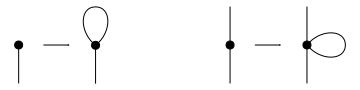
\includegraphics[width=4in]{loop-addition.png}
\item $\edgedouble$ bigon-creation edge doubling duplicates an existing edge joining vertices of degree $< 4$ so as to create a new bigon face, as below.\\
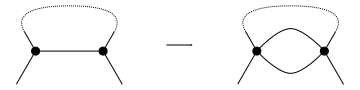
\includegraphics[width=4in]{edge-duplication-non-cut.png}
\item $\cutedgedouble$ cut-edge doubling also duplicates an existing edge joining vertices of degree $<4$, but requires that this edge separate the graph into two connected components. In this case, there is a different way to insert the edge which does not create a bigon with the existing edge. The operation is shown below.\\
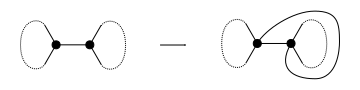
\includegraphics[width=4in]{edge-duplication-cut}
\item $\pairinsert$ pair insertion adds a pair of edges simultaneously, joining two vertices of degree 2 which are both on two faces of the embedding, as below.\\
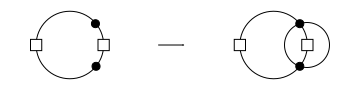
\includegraphics[width=4in]{pair-insertion}
\end{itemize}
\end{definition}

We can now show

\begin{proposition}
Every connected $4$-regular embedded planar (multi)graph $G$ can be obtained from a connected, embedded planar simple graph of vertex degree $\leq 4$ $G_0$ by a series of $\loopinsert$, $\edgedouble$, $\cutedgedouble$, and $\pairinsert$ expansions. 

Equivalently, any connected $4$-regular embedded planar (multi)graph $G$ can be reduced to a connected embedded planar simple graph $G_0$ of vertex degree $\leq 4$ by a series of $\loopinsert$, $\edgedouble$, $\cutedgedouble$, and $\pairinsert$ reductions. The embedded isomorphism type of $G_0$ is determined by the  embedded isomorphism type of $G$ (the order in which the reductions are performed doesn't matter). 
\end{proposition}

An illustration of the process we describe is 
\begin{center}
\includegraphics[width=4in]{expansion-from-simple-graph}
\end{center}

\begin{proof} 
We will prove the second statement, reducing in stages from some $G_n = G$ to $G_0$ by performing one reduction at each step. The number of steps we can perform is clearly finite, since each reduces the number of edges by at least one. So suppose we are at stage $G_i$. If there are no loop or multiple edges, we're done, and this is the simple graph $G_0$. 

If there is a loop edge, we can remove it with a $\loopinsert$ move. If there is a multiple edge, we must consider several cases. We can think of each vertex of $G_i$ as retaining a list of 4 connection points, ordered counterclockwise, from the initial embedding of $G$. Since we have performed some reductions already, some of these may be empty, but at least two are filled at each end of the multiple edge. Pick one vertex of the multiple edge and call it $v$ and the other vertex $w$.

If the edge multiplicity is four, we have the trivial 2-crossing diagram of overlapping circles. We can ignore this case. If the edge multiplicity is three or two, there is more work to do.

So there is at least one connection point on $v$ which is not occupied by a copy of the multiple edge followed immediately by a connection point which is occupied by a copy $e$ of the multiple edge. Without loss of generality, we'll call $e$ the \emph{base copy} of the multiple edge, and its connection point to at $v$ position $0$ around $v$. The remaining connection points will be numbered $1$, $2$, and $3$. By construction, the edge joined to $v$ at position $3$ (if any) is not connected to $w$. 

We can label the other end of the base copy $e$ position $a$ on the second vertex $w$, and label the other positions $b$, $c$, and $d$, again counterclockwise. If the edge multiplicity is three, only one of these positions is unoccupied by a copy of the multiple edge. Looking at the three cases (below), we can see that by parity, it must be position $b$, and the pair of copies $0a$ and $2c$ of the multiple edge can be removed by a $\pairinsert$ operation.
\begin{center}
\includegraphics[width=4in]{multiplicity-three}\\
By parity, because we came from a 4-regular embedded planar graph only the leftmost case can occur at any stage in the reduction process.
\end{center}
We have now disposed of the case where edge multiplicity is three. If edge multiplicity is two, there is one edge unaccounted for, which joins either position $1$ or $2$ on vertex $v$ to position $b$, $c$, or $d$ on vertex $w$. Therefore, there are six cases to address. We consider them in order, starting with the $1x$ configurations.

\begin{itemize}
\item 
\begin{tabular}{m{1in}m{3in}m{1in}}
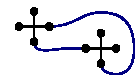
\includegraphics[width=0.9in]{1-b-configuration}
&
In the $1b$ configuration, the multiple edge forms a 2-cycle dividing the portion of the graph $G$ connected to $cd$ from the portion connected to $23$. Deleting $1b$ requires a $\cutedgedouble$ move, and the remaining base edge is a cut edge of all further-reduced $G_i$, as shown at right.
&
\includegraphics[width=0.9in]{1-b-target}
\end{tabular}
\item 
\begin{tabular}{m{1in}m{3in}}
\includegraphics[width=1in]{1-c-configuration}
&
The $1c$ configuration is forbidden by parity. 
\end{tabular}
\item 
\begin{tabular}{m{1in}m{3in}m{1in}}
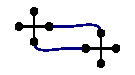
\includegraphics[width=0.9in]{1-d-configuration}
&
In the $1d$ configuration, the multiple edge forms a bigon face. Deleting $1d$ uses an $\edgedouble$ reduction, and yields the configuration at right. The remaining base edge may or may not be a cut edge of the further $G_i$.
&
\includegraphics[width=0.9in]{1-d-target}
\end{tabular}
\end{itemize}
One might think that the $2x$ configurations are simply rearrangements of those above, but this is not true. A genuinely new case arises for $2c$.
\begin{itemize}
\item 
\begin{tabular}{m{1in}m{3in}}
\includegraphics[width=0.9in]{2-b-configuration}
&
The $2b$ configuration is forbidden by parity.
\end{tabular}
\item 
\begin{tabular}{m{1in}m{3in}m{1in}}
\includegraphics[width=1in]{2-c-configuration}
&
In the $2c$ configuration, by parity, the graph $G$ must have connected $1$ and $d$ and also $3$ and $b$. None of our moves change the connectivity of the graph (because we never delete all copies of a multiple edge), so the current graph $G_i$ still joins these pairs of connection points. This means that we are in position for an $\pairinsert$ pair reduction, resulting in the graph at right.
&
\includegraphics[width=1in]{2-c-target}
\end{tabular}
\item 
\begin{tabular}{m{1in}m{3in}}
\includegraphics[width=0.9in]{2-d-configuration}
&
The $2d$ configuration is forbidden by parity.
\end{tabular}
\end{itemize}
Along the way, our analysis has been almost entirely local: we need only consider a single vertex to decide whether we can apply an $\loopinsert$ reduction and a pair of vertices to decide on $\edgedouble$, $\cutedgedouble$, and $\pairinsert$ operations. To show that order of operations doesn't matter, we need to show that whether or not we can apply these operations does not depend on which reductions have already been performed.

The three copies of a multiplicity three edge must bound two bigons, and this does not change as we reduce other edges. Therefore, the $\pairinsert$ move is always available for all multiplicity three edges.

Whether a multiplicity two edge is eligible for an $\edgedouble$ move depends only on the positions of the ends of the multiple copies on their vertices, which doesn't change as we reduce. Therefore, this operation can always be performed (or is always forbidden), regardless of which reductions have already been performed.

Whether a multiplicity two edge is eligible for a $\cutedgedouble$ or $\pairinsert$ operation depends not only on the positions of ends of edges on their vertices, but also on the connectivity of the (reduced) graph. However, as we noted above, the connectivity of the graph doesn't change as we perform reductions.

It is clear that the isomorphism type of $G_0$ does not depend on the order of reduction-- after all, in the end we are simply reducing the multiplicity of multiple edges of the edge. 

It takes only a moment longer to realize that the embedding of $G_0$ is determined as well-- this embedding is determined by the cyclic order of (surviving) edges around their vertices. We will have deleted some edges from many of these vertices by the time we reach $G_0$, potentially leaving many empty connections. However, the cyclic order of the surviving edges won't be affected by the order in which these connections were emptied. 

One might worry that the choice of \emph{which}\footnote{Remember that the choice of ``base edge'' was arbitrary.} copy of an edge of multiplicity two to delete could affect the embedded isomorphism type after an $\edgedouble$ or $\cutedgedouble$ reduction, but it's easy to check that the two possible reduced configurations are (embedded) graph isomorphic by looking at the pictures above. 
\end{proof}


plantri and the plantri theorem
reduction theorem for shadows
reduction for diagrams



\section{Classifying knot types}

homfly
mathematica
snappy

\section{Results}

giant pictures, compared with tait's classification
our distributions
monogon and bigon fractions
degree of alternatingness
universal properties? comparison with distribution from ERPs, lattice walks, and petaluma.

\section{Future Directions}

transitions, unknotting number and so forth.

\end{document}
